\documentclass[../../../Main.tex]{subfiles}
\begin{document}

The implemented algorithm is one step Q-learning.
The AI views the world as a graph structure as to accommodate a Voroni map. This is also simplifies
number of states necessary as the robot position can be represented as a node in the graph as opposed
to a $x$ and $y$ coordinate.
The AI is never penalized for the travel time between nodes, instead the episode will instead just
end. This is done as to not include the time in the state thus keeping the maximum number of states 
to a minimum.
As the time is not a part of the state, the implementation will need to have a discount factor less
than one, as any node with a big number of marbles will have to great a gravitational pull, even if
it is impossible to reach with the allotted time. This gives the AI a bias towards an immediate
reward over future rewards with low/no intermediate rewards.


\subsubsection{Implementation}%
\label{ssub:implementation}
The implementation of an episode can be seen in listing \ref{lst:q:episode}, minus a couple of
\texttt{constexpr} for debug purposes. This listing is shown to emphasize the fact that the AI
does not have any concept of time, and that the time is resolved solely by the allotted time
limit and the cost of each action which is provided by the graph structure on line 6 in the listing.

\lstinputlisting[%
caption=Implementation of an episode.,
label=lst:q:episode,
firstline=76,
lastline=85,
language=c++
]
{\main/afsnit/ai/q_learning/Q_Agent.cpp}

\subsubsection{Definition of states}%
\label{ssub:states}

As previously mentioned the time is not a part the AI's states. It has been attempted keep the states
as simple as possible and thereby the maximum number of states as low as possible. This is done to reduce
the number of episodes needed before the AI converges, due to limited hardware availability.

Since the task is to collect marbles the AI should not be rewarded for going to a node that has
already been cleared. The AI should therefor be able to be certain whether or not a node has been visited
as this should be an important part of its decision making process. To ensure the markovian property
the state should then contain the visit status of all available nodes.

The state should very clearly also contain current position. This will be done via the current
node id and does not interfere with the markovian property of the state.

The theoretical maximum number of states is $n\cdot 2^{n-1}$. This maximum will only be reach if
all nodes can reach all nodes, but this will rarely be the case.


%\begin{figure}[h]
%	\centering
%	%\def\svgwidth{0.4\columnwidth}
%	\subfloat[Caption]{
%		\includesvg[\main/afsnit/ai/q_learning/img/]{node_pos_arg_1}
%	}
%	\subfloat[Caption]{
%		\includesvg[\main/afsnit/ai/q_learning/img/]{node_pos_arg_2}
%	}
%\end{figure}

\subsubsection{Experimental procedure}%
\label{ssub:experimental_procedure}

To test the AI's ability to learn it is tested in simple environments designed to test a single
aspect of its decision making process. These tests are also used to determine which combination of
exploration factor and learning rate is most optimal for the AI to learn the best route in its given
environment.

\paragraph{The circle test}%
\label{par:the_circle_test}

is designed to test that the ai will take the most efficient path given that all nodes contain
the same amount of marbles.
The ai is tested on map, where all nodes are placed in a circle as shown in figure
\ref{fig:q:circle_test}. The ai is able to reach all other nodes from each node and it is not
given enough time to reach all nodes.

\begin{figure}[h]
	\center
	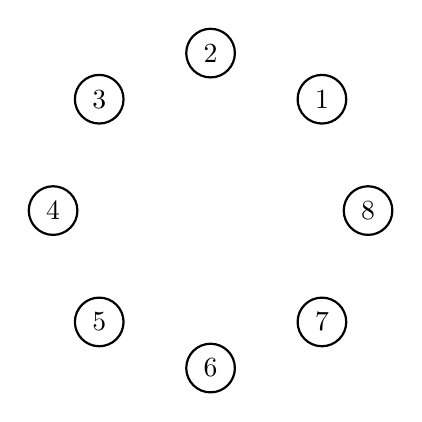
\begin{tikzpicture}
		\foreach \a in {1,...,8}{
			\draw(\a*360/8: 2cm) node[shape=circle,thick,draw]{\a};
		}
	\end{tikzpicture}
	\caption{Example layout of circle test map}
	\label{fig:q:circle_test}
\end{figure}

The AI is run for 100.000 episodes with varying $\epsilon$ and $\alpha$ parameters to see with which
parameters the AI will have the best performance. The performance is measured by how many marbles
the AI collects before the time runs out.

The result of this test with 20 nodes can be seen in figure \ref{fig:q:circ_10000} and
\ref{fig:q:circ_100000}.

\paragraph{The patience test}%
\label{par:the_patience_test}

is designed to test how well the AI handles overcoming multiple nodes with no marbles and then
a great boon of marbles at the end versus a trail of nodes with low marble yield. The
layout of the test environment can be seen in figure \ref{fig:q:patience_test}.
For this this test give a worth while result the amount of marbles at the boon, should account
for the discount factor($\gamma$), as the result otherwise always will show that the trail is the most
worth while path.

\begin{figure}[h]
	\center
	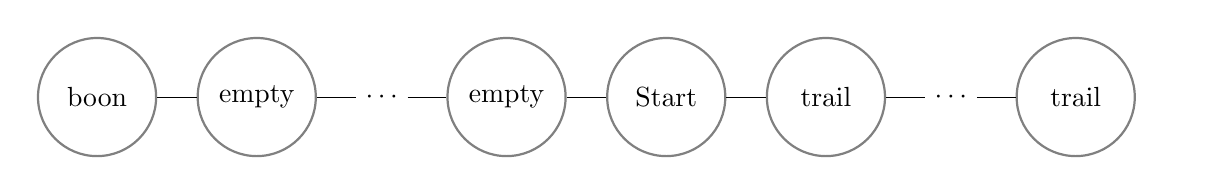
\begin{tikzpicture}[no/.style={minimum size=1.5cm,circle,thick,draw=black!50}]
			\matrix[row sep=1mm,column sep=5mm] {
				\node(p1)[no] {boon};&
				\node(p2)[no] {empty};&
				\node(p3) {$\cdots$ };&
				\node(p4)[no] {empty};&
				\node(p5)[no] {Start};&
				\node(p6)[no] {trail};&
				\node(p7) {$\cdots$ };&
				\node(p8)[no] {trail};&
				\\ };
				\draw (p1) -- (p2) -- (p3) -- (p4) -- (p5) -- (p6) -- (p7) -- (p8);
	\end{tikzpicture}
	\caption{Exmaple layout of patience test}
	\label{fig:q:patience_test}
\end{figure}

\subsubsection{Test results}%
\label{ssub:test_results}

\begin{figure}[h]
  \centering
	\makebox[\textwidth][c]{
		\subfloat[Side view]{
			\def\svgwidth{0.7\textwidth}
			\includesvg[\main/afsnit/ai/q_learning/img/]{CircleTestSideView}
		}
		\subfloat[Top view]{
			\def\svgwidth{0.7\textwidth}
			\includesvg[\main/afsnit/ai/q_learning/img/]{CircleTestTopView}
		}
	}
  \caption{Circle test results after 10000 episodes}
	\label{fig:q:circ_10000}
\end{figure}

\begin{figure}[h]
  \centering
	\makebox[\textwidth][c]{
		\subfloat[Side view]{
			\def\svgwidth{0.7\textwidth}
			\includesvg[\main/afsnit/ai/q_learning/img/]{CircleTestSideView100000}
		}
		\subfloat[Top view]{
			\def\svgwidth{0.7\textwidth}
			\includesvg[\main/afsnit/ai/q_learning/img/]{CircleTestTopView100000}
		}
	}
  \caption{Circle test results after 100000 episodes}
	\label{fig:q:circ_100000}
\end{figure}
\paragraph{The result of the circle test}%
\label{par:the_result_of_the_circle_test}

show that the  ai will learn the best route if it has a learning rate of approximately 0.3 and
a exploration factor of approximately 0.8 under these conditions. These tests have been conducted
with 20 nodes with 1 marble each.

The result of the patience test are not shown as the results show that if the discount factor is
accounted for the AI will always go for the boon.

\paragraph{The result of the patience test}%
\label{par:the_result_of_the_patience_test}
are not shown as the results show that if the discount factor is
accounted for the ai will always go for the boon. This is expected, but it is good to verify.

\subsubsection{Discussion \& Conclusion}%
\label{ssub:conclussion}

The ai was not tested on a map, but tests show that the ai behaves as expected and it therefore
reasonable to assume that the ai will have a good performance in an actual map.\\
As mentioned in regards to the patience test, the ai will have a bias towards immediate rewards over
future rewards, this could be improved with n-step Q-learning or montecarlo learning.
	
\end{document}
